\subsection{Giao diện tạo mới workspace}

\begin{figure}[H]
    \centering
    
\includegraphics[ width = 0.5\linewidth]{Content/Hiện thực hệ thống/documents/Hiện thực giao diện người dùng/images/DropdownMenu.png}
    \vspace{0.5cm}
    \caption{Dropdown menu}
    \label{fig: Giao diện dropdown menu của mỗi item workspace}
\end{figure}

\begin{figure}[H]
    \centering
    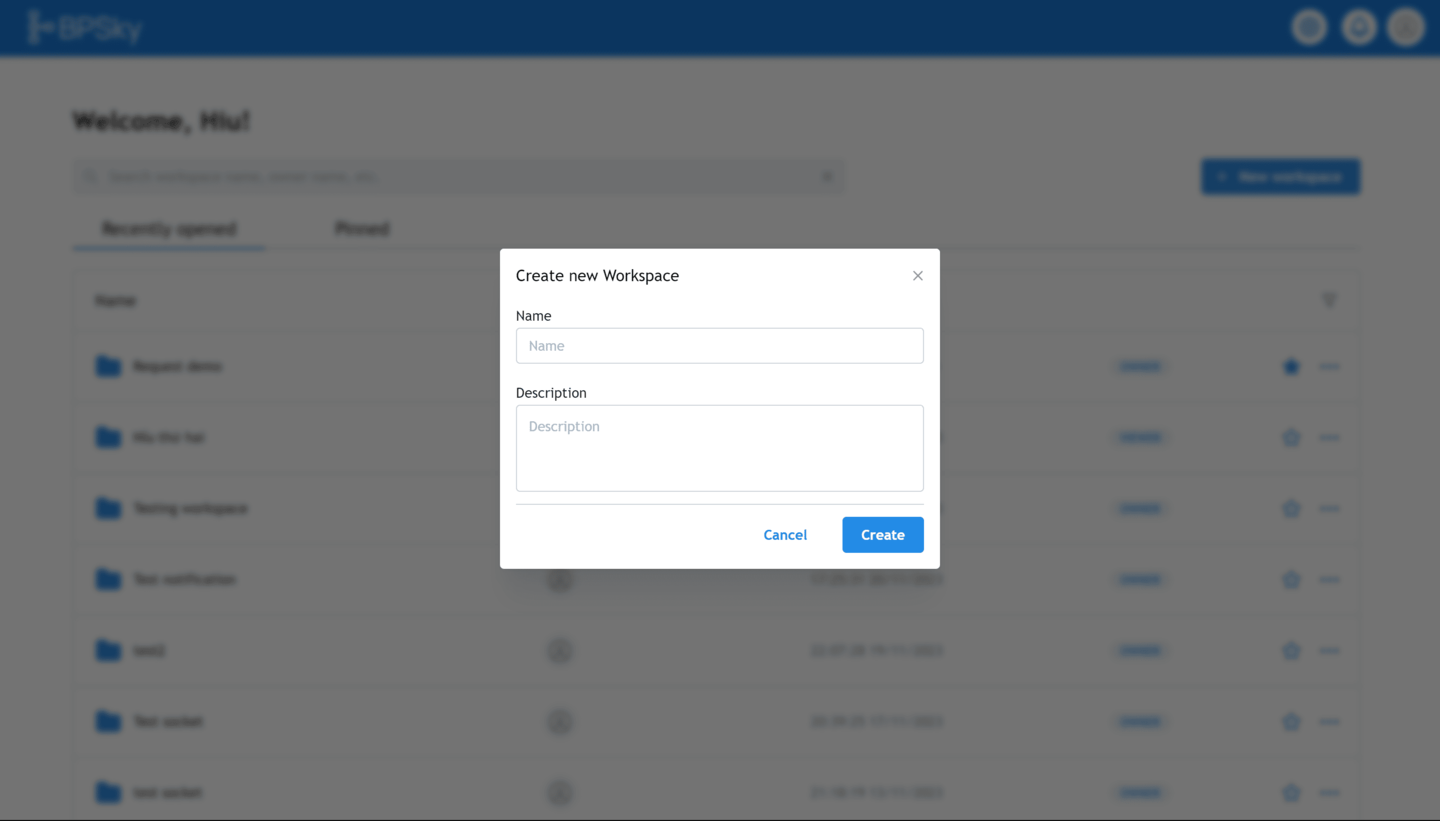
\includegraphics[ width = \linewidth]{Content/Hiện thực hệ thống/documents/Hiện thực giao diện người dùng/images/CreateModal.png}
    \vspace{0.5cm}
    \caption{Giao diện create modal khi người dùng tạo mới workspace}
    \label{fig: Giao diện create modal khi người dùng tạo mới workspace}
\end{figure}

Người dùng có thể tạo mới workspace bằng cách chọn "Create new workspace" từ dropdown menu. Sau khi chọn, hệ thống sẽ hiển thị giao diện create modal như hình \ref{fig: Giao diện create modal khi người dùng tạo mới workspace}. Tại đây, người dùng có thể nhập tên và mô tả cho workspace. Sau khi hoàn tất, người dùng có thể chọn "Create" để tạo mới workspace hoặc "Cancel" để hủy thao tác.